\documentclass[11pt,compress,t,notes=noshow, xcolor=table]{beamer}
\usepackage[]{graphicx}\usepackage[]{color}
% maxwidth is the original width if it is less than linewidth
% otherwise use linewidth (to make sure the graphics do not exceed the margin)
\makeatletter
\def\maxwidth{ %
  \ifdim\Gin@nat@width>\linewidth
    \linewidth
  \else
    \Gin@nat@width
  \fi
}
\makeatother

\newcommand{\citebutton}[2]{%
\beamergotobutton{\href{#2}{#1}}%
}

\newcommand{\blu}[1]{\textcolor{blue}{#1}}
\newcommand{\org}[1]{\textcolor{orange}{#1}}
\newcommand{\ques}{\textbf{\textcolor{red}{Question:  }}}
\newcommand{\questionssofar}{\begin{frame}\frametitle{Any questions?}\end{frame}}

\newcommand\warning{%
 \makebox[1.4em][c]{%
 \makebox[0pt][c]{\raisebox{.1em}{\scriptsize!}}%
 \makebox[0pt][c]{\color{red}\normalsize$\bigtriangleup$}}}%

\definecolor{fgcolor}{rgb}{0.345, 0.345, 0.345}
\newcommand{\hlnum}[1]{\textcolor[rgb]{0.686,0.059,0.569}{#1}}%
\newcommand{\hlstr}[1]{\textcolor[rgb]{0.192,0.494,0.8}{#1}}%
\newcommand{\hlcom}[1]{\textcolor[rgb]{0.678,0.584,0.686}{\textit{#1}}}%
\newcommand{\hlopt}[1]{\textcolor[rgb]{0,0,0}{#1}}%
\newcommand{\hlstd}[1]{\textcolor[rgb]{0.345,0.345,0.345}{#1}}%
\newcommand{\hlkwa}[1]{\textcolor[rgb]{0.161,0.373,0.58}{\textbf{#1}}}%
\newcommand{\hlkwb}[1]{\textcolor[rgb]{0.69,0.353,0.396}{#1}}%
\newcommand{\hlkwc}[1]{\textcolor[rgb]{0.333,0.667,0.333}{#1}}%
\newcommand{\hlkwd}[1]{\textcolor[rgb]{0.737,0.353,0.396}{\textbf{#1}}}%
\let\hlipl\hlkwb

\usepackage{framed}
\makeatletter
\newenvironment{kframe}{%
 \def\at@end@of@kframe{}%
 \ifinner\ifhmode%
  \def\at@end@of@kframe{\end{minipage}}%
  \begin{minipage}{\columnwidth}%
 \fi\fi%
 \def\FrameCommand##1{\hskip\@totalleftmargin \hskip-\fboxsep
 \colorbox{shadecolor}{##1}\hskip-\fboxsep
     % There is no \\@totalrightmargin, so:
     \hskip-\linewidth \hskip-\@totalleftmargin \hskip\columnwidth}%
 \MakeFramed {\advance\hsize-\width
   \@totalleftmargin\z@ \linewidth\hsize
   \@setminipage}}%
 {\par\unskip\endMakeFramed%
 \at@end@of@kframe}
\makeatother

\definecolor{shadecolor}{rgb}{.97, .97, .97}
\definecolor{messagecolor}{rgb}{0, 0, 0}
\definecolor{warningcolor}{rgb}{1, 0, 1}
\definecolor{errorcolor}{rgb}{1, 0, 0}
\newenvironment{knitrout}{}{} % an empty environment to be redefined in TeX

\usepackage{alltt}
\newcommand{\SweaveOpts}[1]{}  % do not interfere with LaTeX
\newcommand{\SweaveInput}[1]{} % because they are not real TeX commands
\newcommand{\Sexpr}[1]{}       % will only be parsed by R
\newcommand{\xmark}{\ding{55}}%


\usepackage[english]{babel}
\usepackage[utf8]{inputenc}

\usepackage{dsfont}
\usepackage{verbatim}
\usepackage{amsmath}
\usepackage{amsfonts}
\usepackage{amssymb}
\usepackage{bm}
\usepackage{csquotes}
\usepackage{multirow}
\usepackage{longtable}
\usepackage{booktabs}
\usepackage{enumerate}
\usepackage[absolute,overlay]{textpos}
\usepackage{psfrag}
\usepackage{algorithm}
\usepackage{algpseudocode}
\usepackage{eqnarray}
\usepackage{arydshln}
\usepackage{tabularx}
\usepackage{placeins}
\usepackage{tikz}
\usepackage{setspace}
\usepackage{colortbl}
\usepackage{mathtools}
\usepackage{wrapfig}
\usepackage{bm}
\usepackage{amsmath}
\usepackage{pifont}

\usetikzlibrary{shapes.multipart,shapes,arrows,automata,positioning,calc,chains,trees, shadows}
\tikzset{
  %Define standard arrow tip
  >=stealth',
  %Define style for boxes
  punkt/.style={
    rectangle,
    rounded corners,
    draw=black, very thick,
    text width=6.5em,
    minimum height=2em,
    text centered},
  % Define arrow style
  pil/.style={
    ->,
    thick,
    shorten <=2pt,
    shorten >=2pt,}
}

\tikzstyle{vec}=[draw, rectangle, fill = white, minimum width=5mm, minimum height=1cm, inner sep = 2pt]

\usepackage{subfig}

% Defines macros and environments
\usepackage{../../style/lmu-lecture}


\let\code=\texttt
\let\proglang=\textsf

\setkeys{Gin}{width=0.9\textwidth}

\setbeamertemplate{frametitle}{\expandafter\uppercase\expandafter\insertframetitle}

\usepackage{bbm}
% basic latex stuff
\newcommand{\pkg}[1]{{\fontseries{b}\selectfont #1}} %fontstyle for R packages
\newcommand{\lz}{\vspace{0.5cm}} %vertical space
\newcommand{\dlz}{\vspace{1cm}} %double vertical space
\newcommand{\oneliner}[1] % Oneliner for important statements
{\begin{block}{}\begin{center}\begin{Large}#1\end{Large}\end{center}\end{block}}


%new environments
\newenvironment{vbframe}  %frame with breaks and verbatim
{
 \begin{frame}[containsverbatim,allowframebreaks]
}
{
\end{frame}
}

\newenvironment{vframe}  %frame with verbatim without breaks (to avoid numbering one slided frames)
{
 \begin{frame}[containsverbatim]
}
{
\end{frame}
}

\newenvironment{blocki}[1]   % itemize block
{
 \begin{block}{#1}\begin{itemize}
}
{
\end{itemize}\end{block}
}

\newenvironment{fragileframe}[2]{  %fragile frame with framebreaks
\begin{frame}[allowframebreaks, fragile, environment = fragileframe]
\frametitle{#1}
#2}
{\end{frame}}


\newcommand{\myframe}[2]{  %short for frame with framebreaks
\begin{frame}[allowframebreaks]
\frametitle{#1}
#2
\end{frame}}

\newcommand{\remark}[1]{
  \textbf{Remark:} #1
}


\newenvironment{deleteframe}
{
\begingroup
\usebackgroundtemplate{
\includegraphics[width=\paperwidth,height=\paperheight]{../style/color/red.png}}
 \begin{frame}
}
{
\end{frame}
\endgroup
}
\newenvironment{simplifyframe}
{
\begingroup
\usebackgroundtemplate{
\includegraphics[width=\paperwidth,height=\paperheight]{../style/color/yellow.png}}
 \begin{frame}
}
{
\end{frame}
\endgroup
}\newenvironment{draftframe}
{
\begingroup
\usebackgroundtemplate{
\includegraphics[width=\paperwidth,height=\paperheight]{../style/color/green.jpg}}
 \begin{frame}
}
{
\end{frame}
\endgroup
}
% https://tex.stackexchange.com/a/261480: textcolor that works in mathmode
\makeatletter
\renewcommand*{\@textcolor}[3]{%
  \protect\leavevmode
  \begingroup
    \color#1{#2}#3%
  \endgroup
}
\makeatother





\input{../../latex-math/basic-math.tex}
\input{../../latex-math/basic-ml.tex}

\def\myblue#1{\textcolor{texblue}{#1}}

\def\qmark{\myblue{?!?}}

%\newcommand{\titlefigure}{figure/gpt_sq.png}
\newcommand{\learninggoals}{
\item Learn to calculate Transformer number of parameters
\item Understand Transformer computation and memory load
\item Learn about Flash Attentions
\item Understand Scaling Laws and Chinchilla
}
\definecolor{texblue}{rgb}{0, 0, 1}
\def\myblue#1{\textcolor{texblue}{#1}}

%\title{LLMs: Parameters, Data, Hardware, Scaling}
\title{}
% \author{}
\institute{\href{https://slds-lmu.github.io/lecture_dl4nlp/}{slds-lmu.github.io/lecture\_dl4nlp}}
\date{}

\begin{document}
\lecturechapter{LLMs: Parameters, Data, Hardware, Scaling}
\lecture{Deep Learning for NLP}


%Notes:
% Slides: https://jasonwei20.github.io/files/FLAN%20talk%20external.pdf
% Check out emergence talk: https://www.youtube.com/watch?v=0SuyDLjNR9g

% LLM Survey: https://arxiv.org/pdf/2303.18223.pdf

% ------------------------------------------------------------------------------

\begin{vbframe}{LLM Parameters: Main Components}

\vfill

\citebutton{Source: Kipply's Blog, 2023}{https://kipp.ly/transformer-param-count/}

\begin{itemize}
    \item Model parameters are half-precision (bfloat16), numbers of 2 bytes
    \item One block (decoder unit) consists of:
		\begin{itemize}
		\item $W_q, W_k, W_v$ matrices which are
    each $n_{heads} \cdot d_{model} \cdot  d_{head}$ and project the input into the queries, keys, and values used in self-attention. 
		\item A $W_0$ matrix which is also $n_{heads} \cdot d_{model} \cdot d_{head}$ for the output of self-attention, before the MLP (feedforward) layer
		\item MLP weights, which are two matrices
    each of ${d_{model}}^2 \cdot 4$. Here
    ``4''  means that the MLP is 4 times the size of the model embedding dimension. 
		\end{itemize}
	\item In most architectures, $d_{model} = n_{heads} \cdot d_{head}$
\end{itemize}

\vfill

\end{vbframe}

% ------------------------------------------------------------------------------

\begin{vbframe}{LLM Parameters: Formula}

\vfill

Combining the above, for one layer/block we get this formula:
\begin{equation*}
\begin{array}{c}
P_{layer} = 3 \cdot d_{model} \cdot n_{heads} \cdot d_{head} + \cdot d_{model} \cdot n_{heads} \cdot d_{head} + 2 \cdot 4 \cdot {d_{model}}^2 \\ [8pt]
 = 4 \cdot d_{model} \cdot n_{heads} \cdot d_{head} + 8 \cdot {d_{model}}^2 \\ [8pt]
 = 4 \cdot d_{model} \cdot d_{model} + 8 \cdot {d_{model}}^2 \\ [8pt]
 = 12 \cdot {d_{model}}^2
\end{array}
\end{equation*}

\vskip5mm

For a LLM of $n$ layers, we get:
\begin{equation*}
\begin{array}{c}
\mbox{total \# parameters\ \ } P = 12 \cdot n_{layers} \cdot {d_{model}}^2
\end{array}
\end{equation*}

\vfill

\end{vbframe}

% ------------------------------------------------------------------------------

\begin{vbframe}{LLM Parameters: Example}

\vfill

GPT-3 Small has:
\begin{equation*}
\begin{array}{l}
n_{params} = 125\,M ~; n_{layers} = 12 ~; d_{model} = 768 ~; n_{heads} = 12 ~; d_{head} = 64 
\end{array}
\end{equation*}

\vskip2mm

GPT-3 Medium has:
\begin{equation*}
\begin{array}{l}
n_{params} = 350\,M ~; n_{layers} = 24 ~; d_{model} = 1024 ~; n_{heads} = 16 ~; d_{head} = 64 
\end{array}
\end{equation*}

\vskip2mm

Applying the above formula we get $\sim$85\,M parameters for GPT-3 Small and $\sim$302\,M parameters for GPT-3 Medium. 



\vfill

\end{vbframe}


\begin{vbframe}{LLM Parameters}

\vfill

\textbf{GPT example}


\vfill

\begin{figure}
\centering
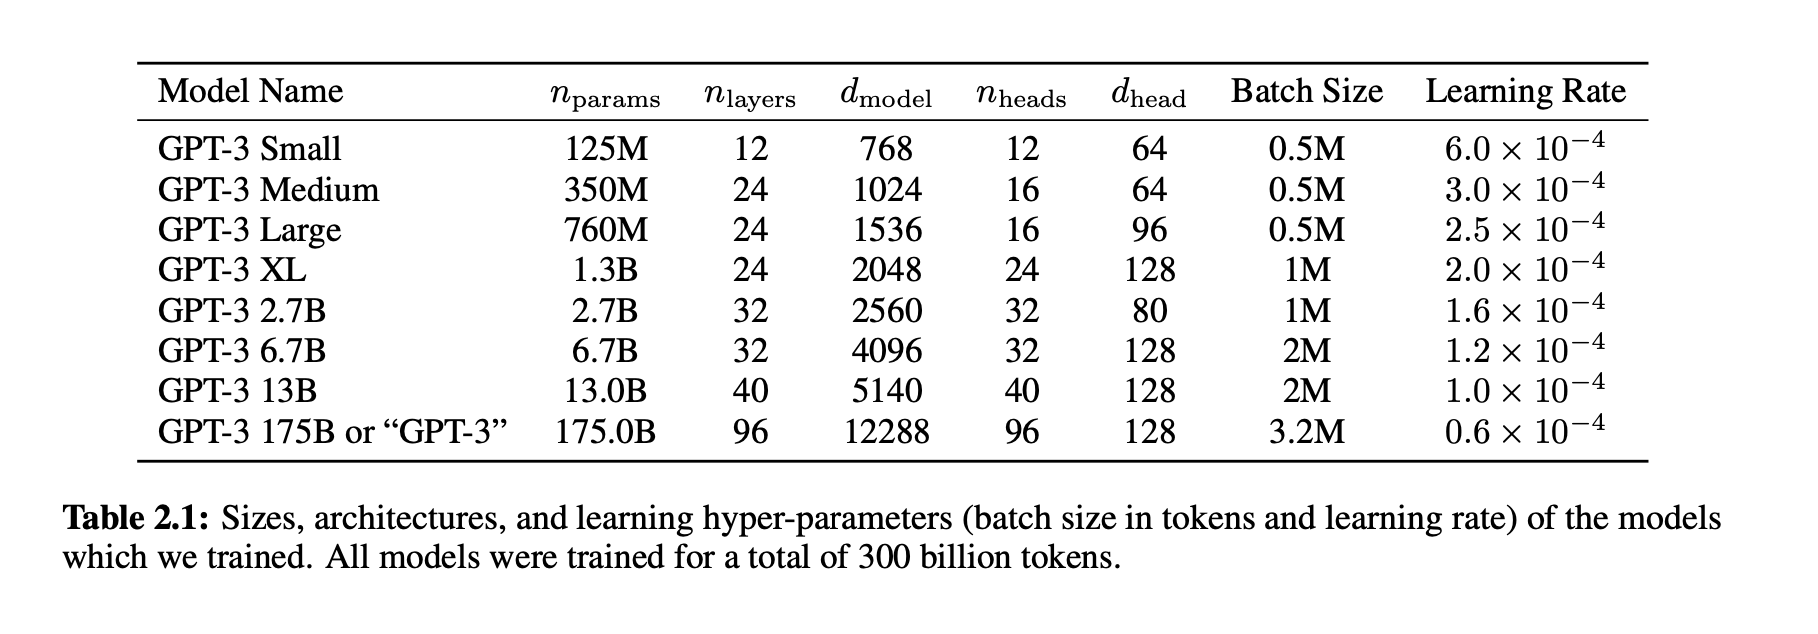
\includegraphics[width = 8cm]{figure/gptsize}
\end{figure}

\begin{itemize}
\item Applying the above formula we get $\sim$85\,M parameters for GPT-3 Small and $\sim$302\,M parameters for GPT-3 Medium. 

\item What are we missing...?!

\end{itemize}



\vfill

\end{vbframe}

% ------------------------------------------------------------------------------

\begin{vbframe}{LLM Parameters: Other Components}

\vfill

Numeric illustration as in BERT-base \\ \vskip5mm

\begin{itemize}
    \item Word Embedding parameters -- 30522 x 768 = 23,440,896
    \item Position Embedding parameters -- 512 x 768 = 393,216
	\item Token Type Embedding parameters -- 2 x 768 = 1536
	\item Embedding Layer Normalization, weight and Bias -- 768 + 768 = 1536
	\item Other model-specific parameters...
\end{itemize}

\vskip5mm

Total Embedding parameters = 23,837,184 \vskip3mm

They do not scale with model size.

\vfill

\end{vbframe}

% ------------------------------------------------------------------------------

\begin{vbframe}{Compute Requirements}

\vfill

\textbf{Basic equation: Cost to train a transformer (decoder) model:}

\vspace{1.5cm}

$$C \approx \tau T = 6 P D$$ 

\vspace{1.5cm}

\centering \citebutton{Source: Quentin et al., 2023}{https://blog.eleuther.ai/transformer-math/}

\vfill

\end{vbframe}

% ------------------------------------------------------------------------------

\begin{vbframe}{Compute Requirements}

\vfill

\textbf{where:}

\begin{itemize}
    \item $C$: No. of floating-point operations (FLOPs) to train the model:\\
          $C = C_{forward} + C_{backward}$
	\item $C_{forward} \approx 2 P D$
	\item $C_{backward} \approx 4 P D$
	\item $\tau$ is throughput of hardware: (No. GPUs) x (FLOPs/GPU)
	\item $T$ is the time spent training the model, in seconds
	\item $P$ is the number of parameters in the model
	\item $D$ is the dataset size (in tokens)
\item $2PD$: ``2'' comes from the multiply-accumulate
          operation used in
          matrix multiplication
          \item $4PD$: backward pass approximately twice
          the compute of the forward pass
          (in the backward pass at each
          layer, gradients have to be calculated for the
          weights at that layer and for the previous layer's
          output, so that the gradient of the previous
          layer's weights can be calculated)
          
\end{itemize}

\vfill

\end{vbframe}

% ------------------------------------------------------------------------------

\begin{vbframe}{Compute Units}

\vfill

$C$  can be measured in different units:\newline

\begin{itemize}
    \item FLOP-seconds which is [Floating Point Ops / Second]
	\begin{itemize}
	    \item We also use multiples GFLOP-seconds, TFLOP-seconds etc.
		\item Other multiples like PFLOP-days are used in papers
		\item 1 PFLOP-day = $10^{15} \cdot 24 \cdot 3600$ FLOP-seconds
	\end{itemize}
	\item GPU-hours which is [No. GPUs] x [Hours]
	\begin{itemize}
	    \item GPU model is also required, since they have different compute capacities
		\item For any GPU model, its Actual FLOPs are always lower than the advertised theoretical FLOPs
	\end{itemize}
\end{itemize}

\vfill

\end{vbframe}

% ------------------------------------------------------------------------------

\begin{vbframe}{Parameter vs Dataset}

\vfill

\begin{itemize}
    \item Model performance depends on number of parameters $P$, but also on number of training tokens $D$
	\item We need to decide about $P$ and $D$, so that we get the best performance within the compute budget
	\item
        Recommended tradeoff between $P$ and $D$ is: $D = 20 P$
	\begin{itemize}
	    \item This is usually true for Chinchilla models \citebutton{Hoffmann et al., 2022}{https://arxiv.org/abs/2203.15556},\\but not for all LLMs
	\end{itemize}
	\item Training a LLM for less than 200 billion tokens is not recommended
	\item Rule of thumb: First determine the upmost inference cost, and then train the biggest model within that boundary.
\end{itemize}

\vfill

\end{vbframe}

% ------------------------------------------------------------------------------

\begin{vbframe}{Memory Requirements}

\vfill

Common questions: \newline

\begin{itemize}
 	\item How big is this model in bytes?
	\item Will it fit/train in my GPUs?
\end{itemize}

\vskip8mm

Model size components: \newline

\begin{itemize}
 	\item Model parameters
	\item Optimizer states
	\item Gradients
	\item Activations
\end{itemize}

\vfill

\end{vbframe}

% ------------------------------------------------------------------------------

\begin{vbframe}{Number Representations}

\vfill

\begin{itemize}
 	\item Pure fp32: single precision floating point number as defined by \citebutton{IEEE 754}{https://en.wikipedia.org/wiki/IEEE_754} standard, takes 32 bits or 4 bytes
 	\item fp16: half precision float number as defined by \citebutton{IEEE\_754-2008}{https://en.wikipedia.org/wiki/IEEE_754-2008_revision}, occupying 16 bits or 2 bytes 
    \item bf16 or brain floating point 16, developed by Google Brain project, occupying 16 bits or 2 bytes
	\item int8: integer from -128 to 127, occupying 8 bits or 1 byte
\end{itemize}

\vfill

\end{vbframe}

% ------------------------------------------------------------------------------

\begin{vbframe}{Model Parameters}

\vfill

Parameter size depends on chosen representation: \newline

\begin{itemize}
 	\item Pure fp32: $Mem_{model} = 4 ~bytes/param \cdot N_{params}$
 	\item fp16 or bf16: $Mem_{model} = 2 ~bytes/param \cdot N_{params}$
	\item int8: $Mem_{model} = 1 ~byte/param \cdot N_{params}$
\end{itemize}

\vskip8mm

It is practically common to use mixed representations: \newline

\begin{itemize}
 	\item fp32 + fp16
	\item fp32 + bf16
\end{itemize}

\vfill

\end{vbframe}

% ------------------------------------------------------------------------------

\begin{vbframe}{Optimizer States}

\vfill

AdamW: $Mem_{AdamW} = 12 ~bytes/param \cdot N_{params}$
\begin{itemize}
 	\item fp32 copy of parameters: 4 bytes/param
 	\item Momentum: 4 bytes/param
	\item Variance: 4 bytes/param
\end{itemize}

\vskip3mm

bitsandbytes (8-bit optimizer): $Mem_{AdamW} = 6 ~bytes/param \cdot N_{params}$
\begin{itemize}
 	\item fp32 copy of parameters: 4 bytes/param
 	\item Momentum: 1 byte/param
	\item Variance: 1 byte/param
\end{itemize}

%\vskip3mm
%
%For AdamW, memory = $ 12 ~bytes/param \cdot N_{params}$
%\begin{itemize}
% 	\item fp32 copy of parameters: 4 bytes/param
% 	\item Momentum: 4 bytes/param
%\end{itemize}

\vfill

\end{vbframe}

% ------------------------------------------------------------------------------

\begin{vbframe}{Gradients}

\vfill

They are usually stored in the same datatype as the model parameters. \newline

Their memory overhead contribution is: \newline


\begin{itemize}
 	\item fp32: $Mem_{grad} = 4 ~bytes/param \cdot N_{params}$
 	\item fp16 or bf16: $Mem_{grad} = 2 ~bytes/param \cdot N_{params}$
	\item int8: $Mem_{grad} = 1 ~byte/param \cdot N_{params}$
\end{itemize}

\vfill

\end{vbframe}

% ------------------------------------------------------------------------------

\begin{vbframe}{Activations}

\vfill

\begin{itemize}
 	\item GPUs are bottlenecked by memory, not FLOPs
 	\item Save GPU memory by recomputing activations of certain layers
	\item Various schemes for selecting which layers to clear
	\item They take some extra memory, but save even more
\end{itemize}

\vskip5mm

Total memory when training \textbf{without} activations: \newline
$Mem_{training} = Mem_{params} + Mem_{opt} + Mem_{grad}$

\vskip5mm

Total memory when training \textbf{using} activations: \newline
$Mem_{training} = Mem_{params} + Mem_{opt} + Mem_{grad} + Mem_{activ}$

\vskip5mm

In the latter case, $Mem_{params}$, $Mem_{opt}$ and $Mem_{grad}$ are significantly smaller than in the former.

\vfill

\end{vbframe}

% ------------------------------------------------------------------------------

\begin{vbframe}{Distributed Training}

\vfill

\begin{itemize}
 	\item Training LLMs faster on many GPUs
 	\item Avoiding OOM issues
	\item \textbf{Data parallelism:} split the data on different model replicas
	\item \textbf{Tensor parallellism:} split model parameters accross GPUs
	\item \textbf{Sharded optimizers:} reduce optimizer overhead by No. GPUs
%	\begin{itemize}
%	 	\item ZeRO (Zero Redundancy Optimizer)
%		\item Requires low extra communication between GPUs
%	 	\item Decreases optimizer memory requirement
%		\item Improves training speed
%\end{itemize}
\end{itemize}

\vfill

\end{vbframe}

% ------------------------------------------------------------------------------

\begin{vbframe}{Data Paralelism}

\vfill

\begin{figure}
	\centering
	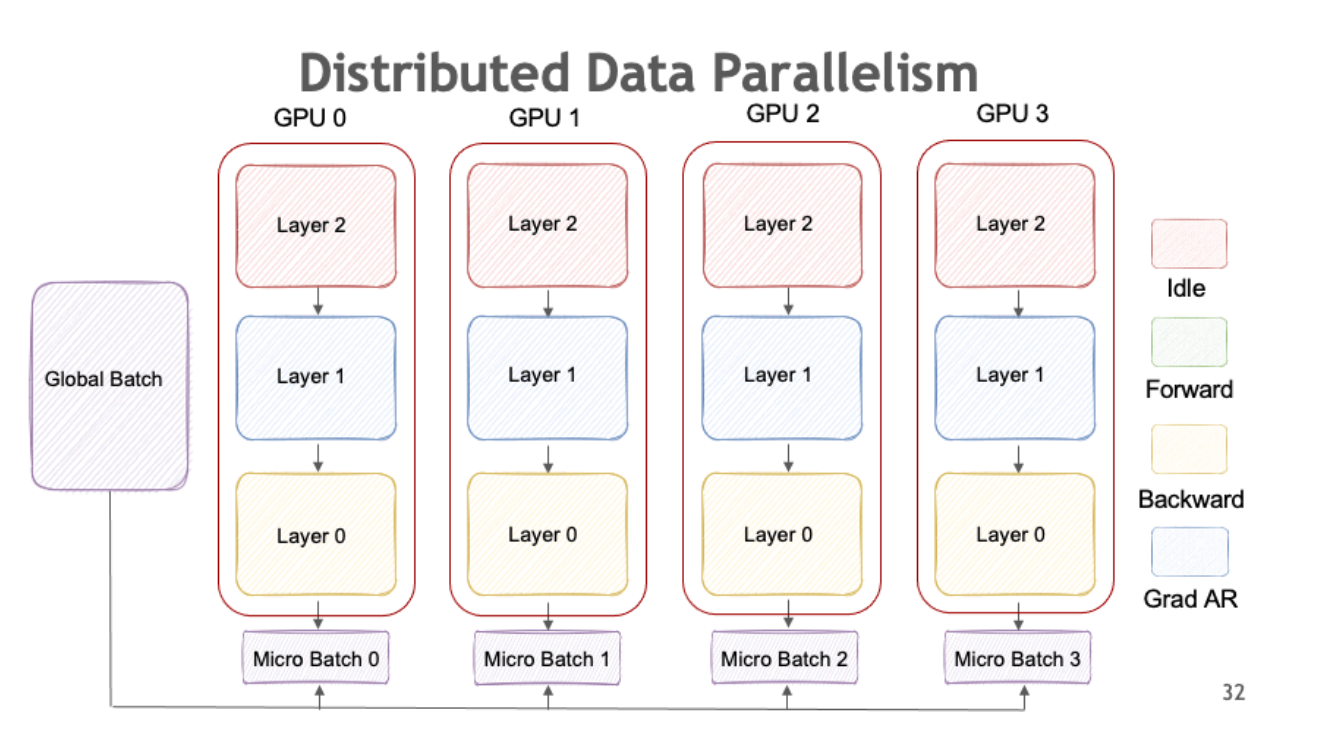
\includegraphics[width = 11cm]{./figure/data_parallel.png} \\ 
	{\footnotesize Source: \href{https://docs.nvidia.com/deeplearning/nemo/user-guide/docs/en/stable/nlp/nemo_megatron/parallelisms.html}{Nvidia}}
\end{figure}

\vfill

\end{vbframe}

% ------------------------------------------------------------------------------

\begin{vbframe}{Tensor Paralelism}

\vfill

\begin{figure}
	\centering
	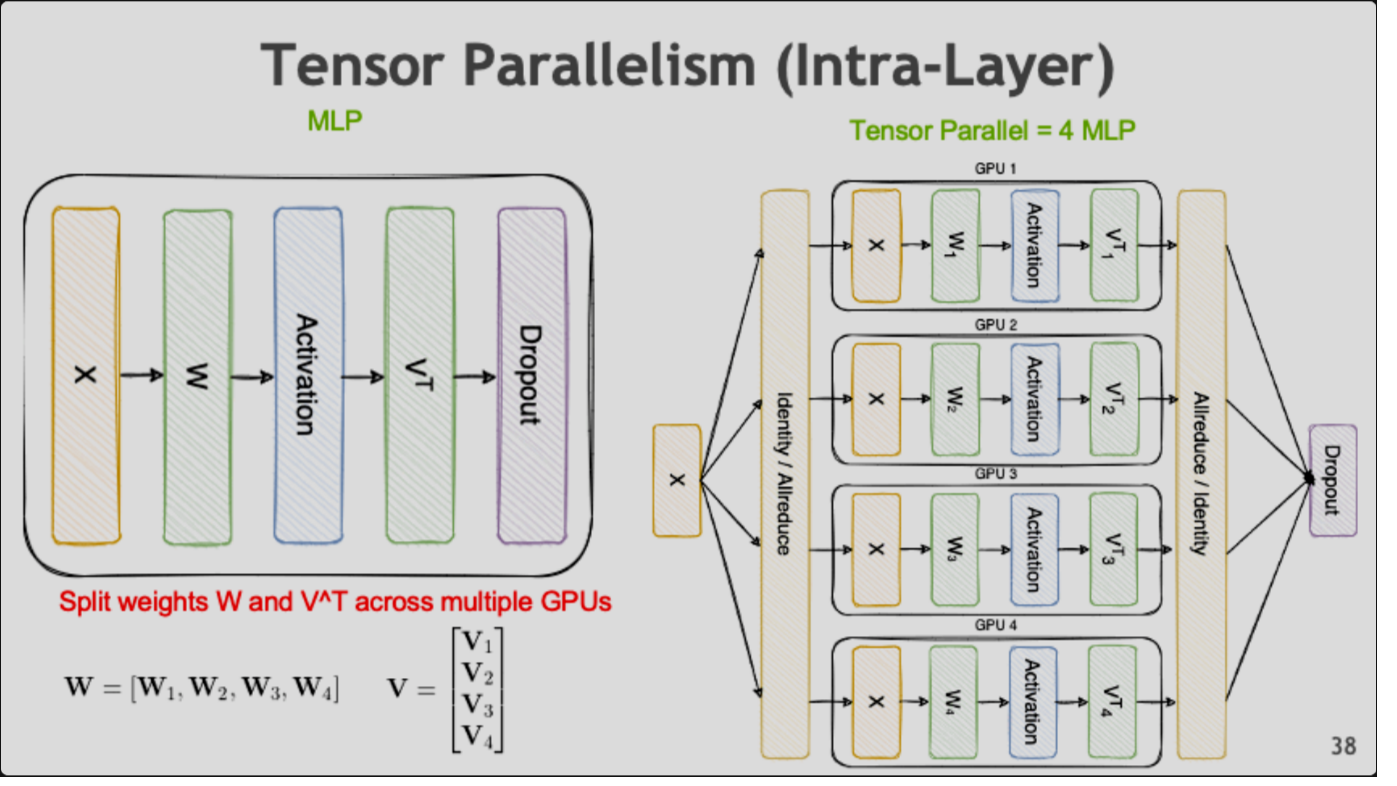
\includegraphics[width = 11cm]{./figure/tensor_paralel.png} \\ 
	{\footnotesize Source: \href{https://docs.nvidia.com/deeplearning/nemo/user-guide/docs/en/stable/nlp/nemo_megatron/parallelisms.html}{Nvidia}}
\end{figure}

\vfill

\end{vbframe}

% ------------------------------------------------------------------------------

%\begin{vbframe}{Zero Redundancy Optimizer}
%
%\vfill
%
%\begin{figure}
%	\centering
%	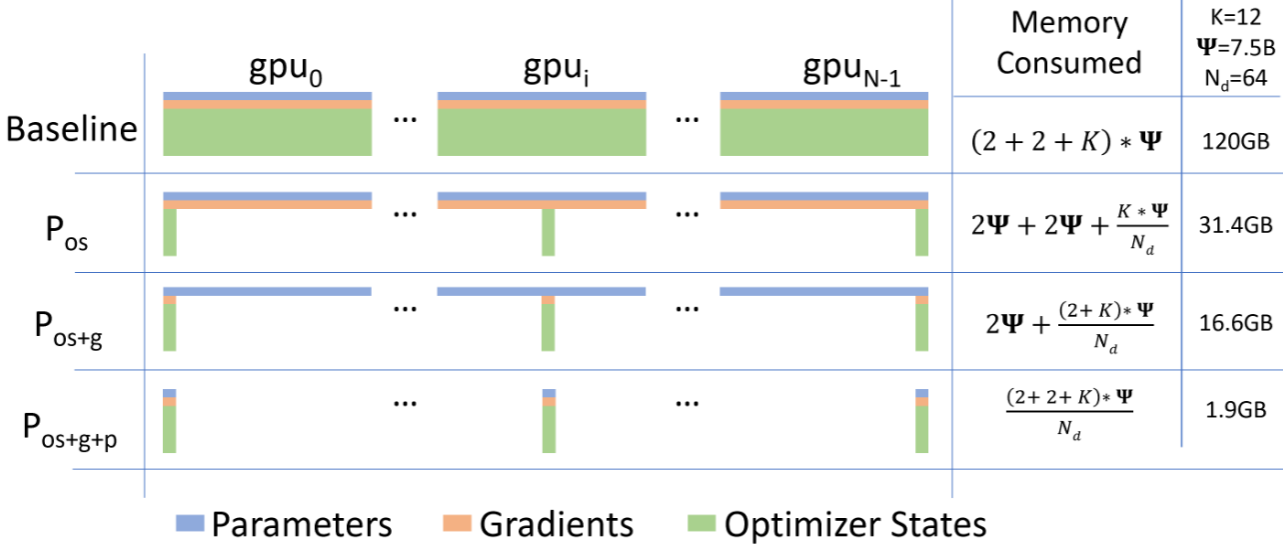
\includegraphics[width = 11cm]{./figure/zero_paralel.png} \\ 
%%%%% \caption{Comparing the per-device memory consumption of model states, with three stages of ZeRO-DP optimizations.}
%  \citebutton{Rajbhandari et al., 2020}{https://arxiv.org/pdf/1910.02054.pdf}
%  
%\end{figure}
%
%\vfill
%
%\end{vbframe}

% ------------------------------------------------------------------------------

\begin{vbframe}{F\MakeLowercase{lash}A\MakeLowercase{ttention}}

\vfill

Fast and Memory-Efficient Exact Attention with IO-Awareness \newline

\begin{itemize}
	\item Fast
	\begin{itemize}
		\item 15\,\% faster than BERT
		\item 3x faster than GPT-2 
		\item 2.4x faster than Megatron-LM
	\end{itemize}
	\item Memory-efficient
	\begin{itemize}
		\item Reducing from $O(\MakeLowercase{n}^2)$ to $O(\MakeLowercase{n})$ 
	\end{itemize}
	\item Exact
	\begin{itemize}
		\item Same as ``vanilla attention'', not an approximation 
	\end{itemize}
	\item IO aware
	\begin{itemize}
		\item Reducing memory load/store operations
	\end{itemize}
\end{itemize}

\vfill

\end{vbframe}

% ------------------------------------------------------------------------------

\begin{vbframe}{GPU Memory Hierarchy}

\vfill

\begin{figure}
	\centering
	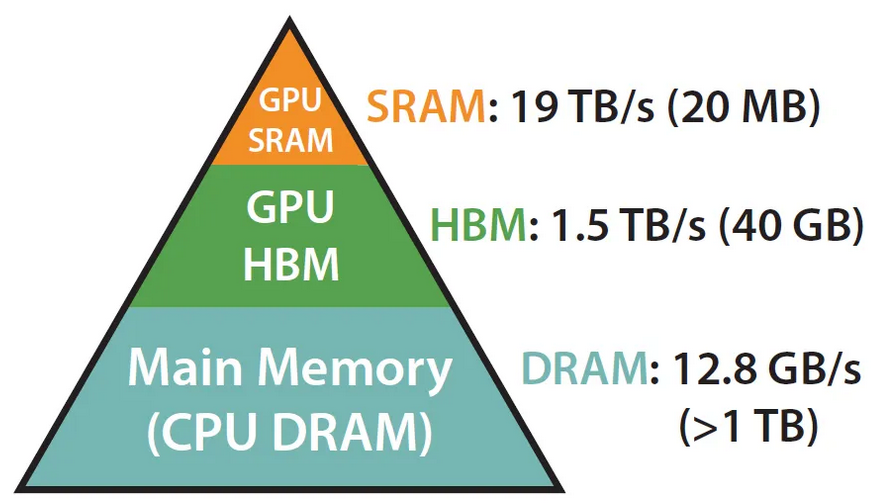
\includegraphics[width = 11cm]{./figure/gpu_mem.png} \\ 
	{\footnotesize Source: \href{https://arxiv.org/abs/2205.14135}{Dao et al. (2022)}}
\end{figure}

\vfill

\end{vbframe}

% ------------------------------------------------------------------------------

\begin{vbframe}{Computing Considerations}

\vfill

\begin{itemize}
	\item GPU compute has been growing faster than memory bandwidth
	\begin{itemize}
		\item GPU has to wait for data
	\end{itemize}
	\item Transformer operations are memory-bound
	\begin{itemize}
		\item Elementwise operations with high memory access
	\end{itemize}
	\item IO aware means reducing memory load/store operations
	\item FlashAttention implements the following:
	\begin{itemize}
		\item Operation fusion to reduce memory access
		\item Tiling or chunking the softmax matrix into blocks
		\item Recomputation for better memory utilization
	\end{itemize}
\end{itemize}

\vfill

\end{vbframe}

% ------------------------------------------------------------------------------

\begin{vbframe}{Operation Fusion}

\vfill

\begin{figure}
	\centering
	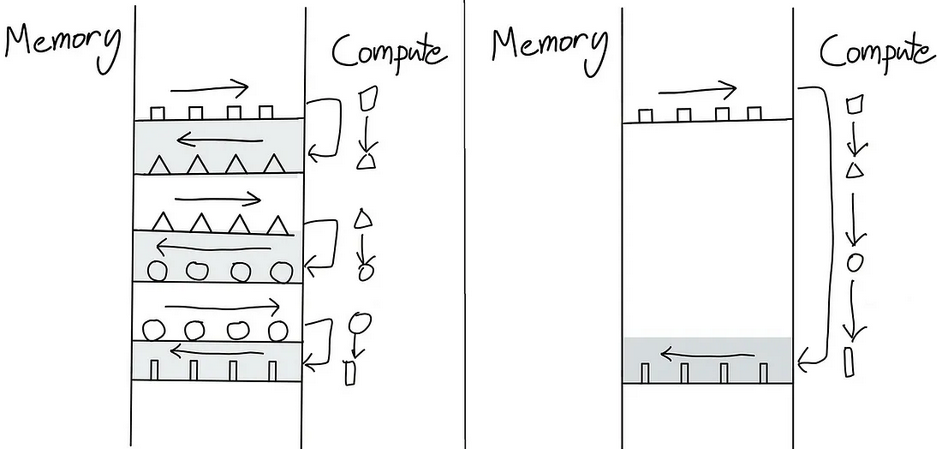
\includegraphics[width = 11cm]{./figure/op_fusion.png} \\ 
	{\footnotesize Source: \href{https://horace.io/brrr_intro.html}{\url{https://horace.io/brrr_intro.html}}}
\end{figure}

\vfill

\end{vbframe}

% ------------------------------------------------------------------------------

\begin{vbframe}{Limitations and Prospects}

\vfill

\begin{itemize}
	\item FlashAttention requires writing attention to CUDA language
	\begin{itemize}
		\item A new CUDA kernel for each new attention implementation
		\item CUDA is lower-level than PyTorch
		\item Implementation may not be transferable accross GPUs
	\end{itemize}
	\item Towards IO-Aware Deep Learning
	\begin{itemize}
		\item Extending beyonde attention
	\end{itemize}
	\item Multi-GPU IO-Aware Methods
	\begin{itemize}
		\item FlashAttention computation may be parallelizable accross multiple GPUs
	\end{itemize}
\end{itemize}

\vfill

\end{vbframe}

% ------------------------------------------------------------------------------

\begin{vbframe}{Scaling Laws}
\href{https://arxiv.org/abs/2001.08361}{\beamergotobutton{Kaplan et al. (2020)}} 

\vfill

\begin{itemize}

	\item Performance depends strongly on scale, weakly on model shape
	\begin{itemize}
	\item Scale means: parameters $N$, data $D$, and compute $C$
	\item Shape means: depth and width
	\end{itemize}

	\item Smooth power laws \qmark
	\begin{itemize}
	\item Performance has power-law relation with each factor $N$, $D$, $C$
	\item When not bottlenecked by the other two 
	\item Trend spanning more than six orders of magnitude
	\end{itemize}

	\item Universality of overfitting \qmark 
	\begin{itemize}
	\item Performance enters regime of diminishing returns if $N$ or $D$ held fixed while the other increases
	%\item Performance penalty depends on $N^{0.74} / D$
	\end{itemize}

\end{itemize}

\vfill

\end{vbframe}

% ------------------------------------------------------------------------------

\begin{vbframe}{Scaling Laws}

\vfill

\begin{itemize}

	\item Universality of training (see figure next
	slide) \qmark
	\begin{itemize}
	\item Training curves follow predictable power-laws
	\item Their parameters are roughly independent of model size
	\item It is possible to predict by extrapolating the early part of the training curve
	\end{itemize}

	\item Transfer improves with test performance \qmark
	\begin{itemize}
	\item When evaluating on text with different distribution from training text, results are strongly correlated to those on the validation set
	\item Transfer to different distribution incurs a constant penalty but improves in line with performance on training set
	\end{itemize}

	\item Sample efficiency \qmark
	\begin{itemize}
	\item Large models are more sample-efficient than small models
	\item They reach same performance with fewer optimization steps
	\end{itemize}

\end{itemize}

\vfill

\end{vbframe}


\begin{vbframe}{Power law (gpt3 paper)}

\vfill

\begin{figure}
	\centering
	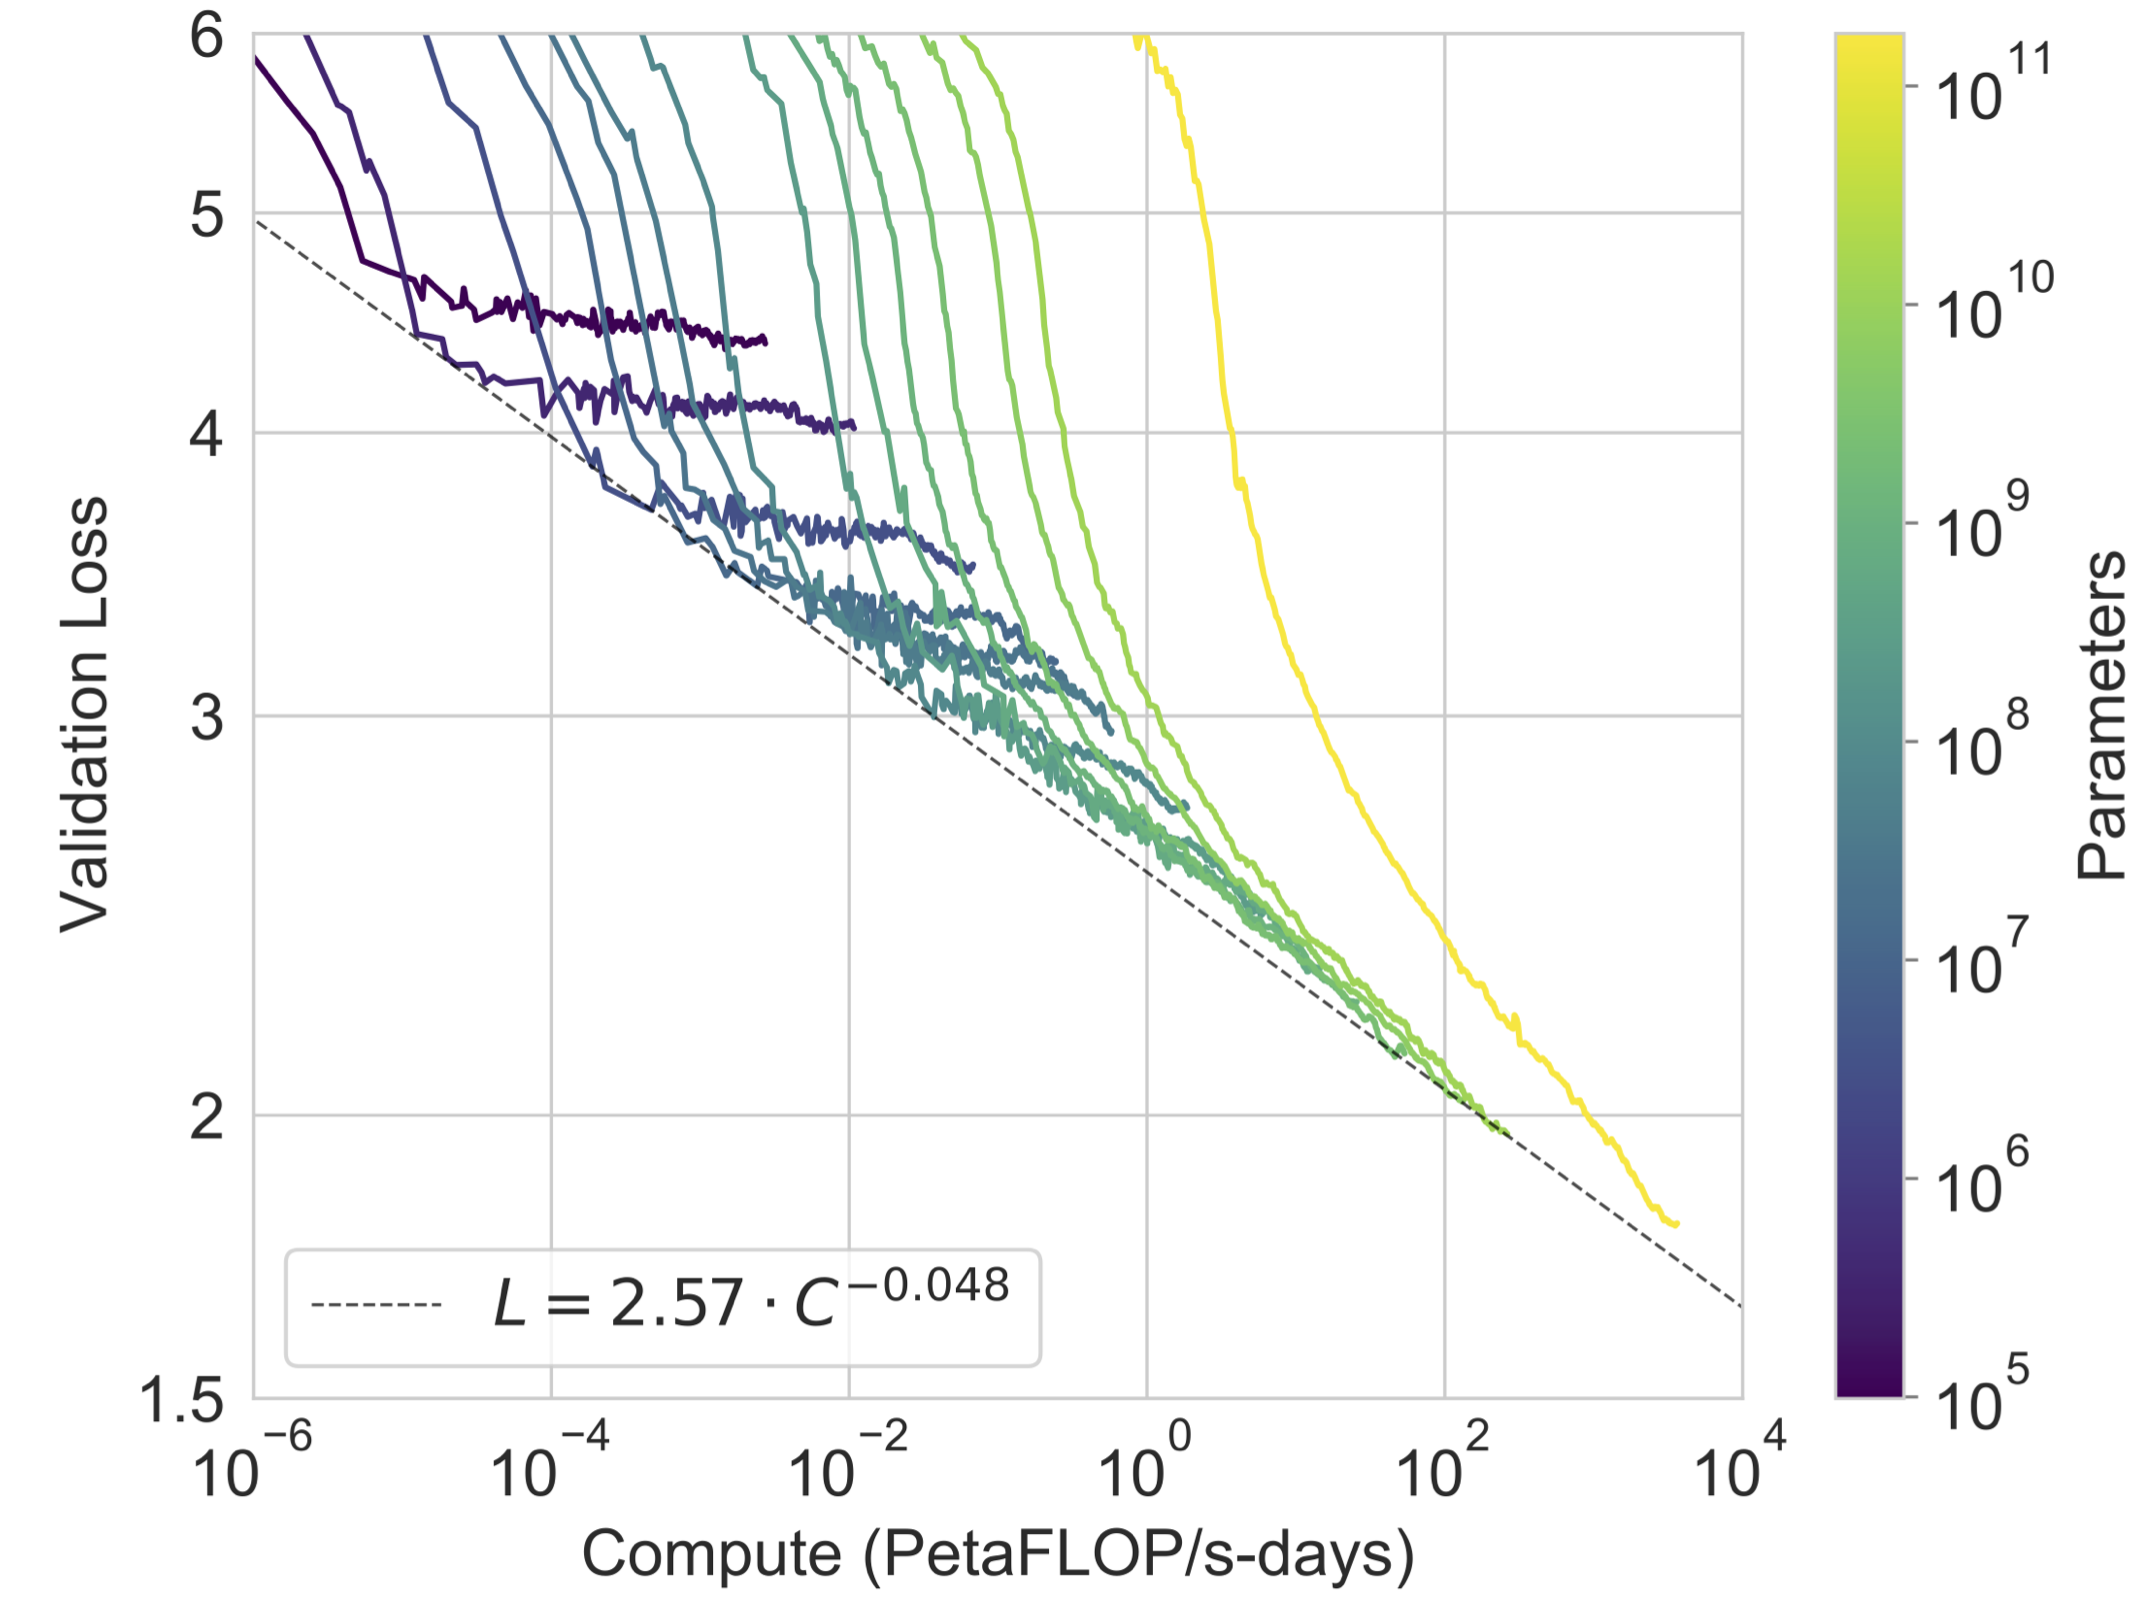
\includegraphics[width = 9cm]{./figure/losscompute}
\end{figure}

\vfill

\end{vbframe}


% ------------------------------------------------------------------------------

\begin{vbframe}{Scaling Laws}

\vfill

\begin{itemize}

	\item Convergence is inefficient
	\begin{itemize}
	\item When $C$ is fixed but $N$ and $D$ are not,
	optimal performance is achieved by training very
	large models and stopping significantly short of
	convergence (QUESTION: why?)  
	\end{itemize}

	\item Optimal batch size \qmark
	\begin{itemize}
%	\item Ideal size is a power of the loss only
	\item $\sim$1-2 million tokens for the largest models 
	\end{itemize}

\end{itemize}

\vskip3mm

\textbf{Larger language models will perform better and be
	more sample efficient than current models. \qmark} 

\vfill

\end{vbframe}


\begin{vbframe}{Scaling law for next word prediction}

\vfill

\begin{itemize}


\item $L(N,D) = 1.61 + \frac{406.4}{N^{0.34}}        + \frac{410.7}{D^{0.28}}$        

\item $L(N,D)$ is cross entropy on new text.
        
	\end{itemize}


\vskip3mm

%\textbf{Larger language models will perform better and be more sample efficient than current models.} 

\vfill

\end{vbframe}

% ------------------------------------------------------------------------------

\begin{vbframe}{Compute-Optimal LLM\MakeLowercase{s}}

Given a fixed FLOPs budget, how should we trade-off model size and text size to optimize performance? \citebutton{Hoffmann et al., 2022}{https://arxiv.org/abs/2203.15556}

\vfill

\begin{itemize}

	\item Find $N$ and $D$ so that $FLOPs(N,D) = C$ and $L(N,D)$ is minimal

	\item Empirically estimated $N$ and $D$ based on 400 models. 
	\begin{itemize}
	\item Ranging from 70\,M to 16\,B parameters
	\item Trained on 5\,B to 400\,B tokens
	\end{itemize}

	\item Different results from those of \citebutton{Kaplan et al., 2020}{https://arxiv.org/abs/2001.08361} 
	\item Results verified using Chinchilla
	\begin{itemize}
	\item Chinchilla has 70\,B parameters and is trained on 1.4\,T tokens
	\item 4x less parameters and 4x more tokens than Gopher
	\item Chinchilla outruns Gopher and has reduced memory footprint and inference cost 
	\end{itemize}

\end{itemize}

\vfill

\end{vbframe}

% ------------------------------------------------------------------------------

\begin{vbframe}{Compute-Optimal LLMs}

\vfill

\begin{figure}
	\centering
	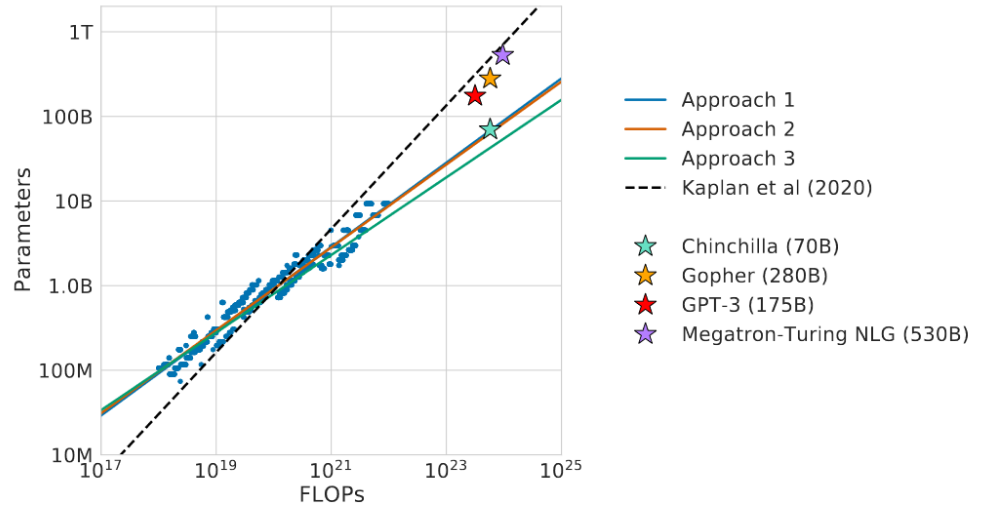
\includegraphics[width = 11cm]{./figure/chinchilla.png} \\ 
	\citebutton{Source: Hoffmann et al., 2022}{https://arxiv.org/abs/2203.15556}
\end{figure}

Given a fixed FLOPs budget,1 how should one trade-off model
size and the number of training tokens? 
We find that all three methods predict that current large
models should be substantially smaller and therefore trained
much longer than is currently done.


\vfill

\end{vbframe}

\begin{vbframe}{Compute-Optimal LLMs (2)}


Given a fixed FLOPs budget,1 how should one trade-off model
size and the number of training tokens? 
We find that all three methods predict that current large
models should be substantially smaller and therefore trained
much longer than is currently done.
Based on our estimated compute-optimal frontier, we predict
that for the compute budget used to train Gopher, an optimal
model should be 4 times smaller, while being training on 4
times more tokens. We verify this by training a more
compute-optimal 70B model, called Chinchilla, on 1.4
trillion tokens. Not only does Chinchilla outperform its
much larger counterpart, Gopher, but its reduced model size
reduces inference cost considerably and greatly facilitates
downstream uses on smaller hardware. The energy cost of a
large language model is amortized through its usage for
inference an fine-tuning. The benefits of a more optimally
trained smaller model, therefore, extend beyond the
immediate benefits of its improved performance.


\vfill

\end{vbframe}

% ------------------------------------------------------------------------------

\begin{vbframe}{Chinchilla and the other LLM\MakeLowercase{s}}

\vfill

\begin{figure}
	\centering
	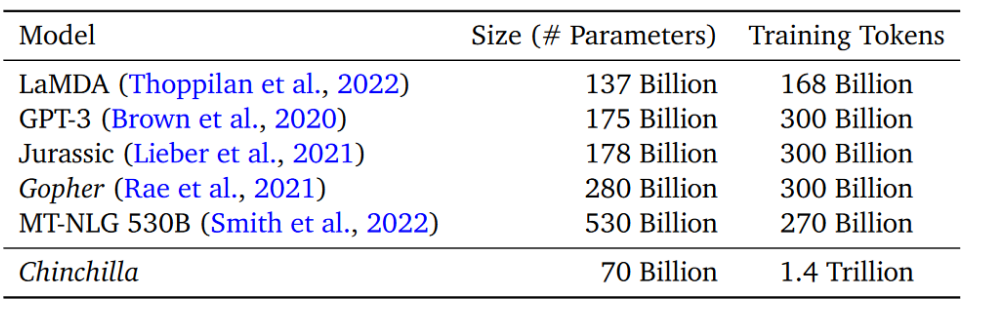
\includegraphics[width = 11cm]{./figure/llm_params.png} \\ 
	\citebutton{Source: Hoffmann et al., 2022}{https://arxiv.org/abs/2203.15556}
\end{figure}

\begin{figure}
	\centering
	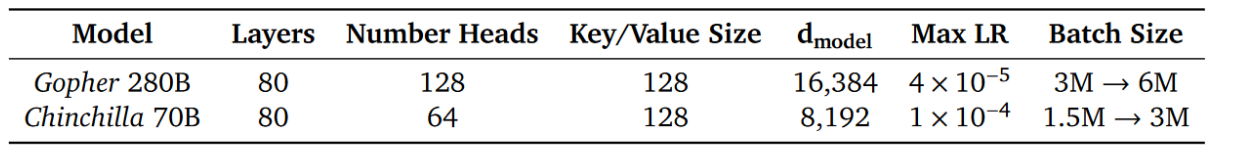
\includegraphics[width = 11cm]{./figure/chinchilla_gopher.png} \\ 
	\citebutton{Source: Hoffmann et al., 2022}{https://arxiv.org/abs/2203.15556}
\end{figure}

\vfill

\end{vbframe}

% ------------------------------------------------------------------------------

\begin{vbframe}{Chinchilla outperforms other LLMs: MMLU}

\vfill

\begin{figure}
	\centering
	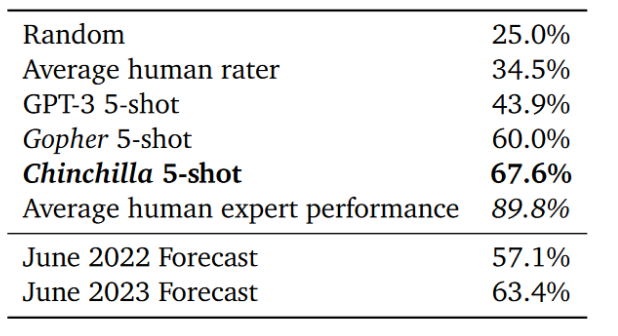
\includegraphics[width = 8cm]{./figure/chinchilla_mmlu.png} \\ 
	\citebutton{Source: Hoffmann et al., 2022}{https://arxiv.org/abs/2203.15556}
\end{figure}

\vfill

\end{vbframe}

% ------------------------------------------------------------------------------

\begin{vbframe}{Chinchilla outperforms other LLMs: QA}

\vfill

\begin{figure}
	\centering
	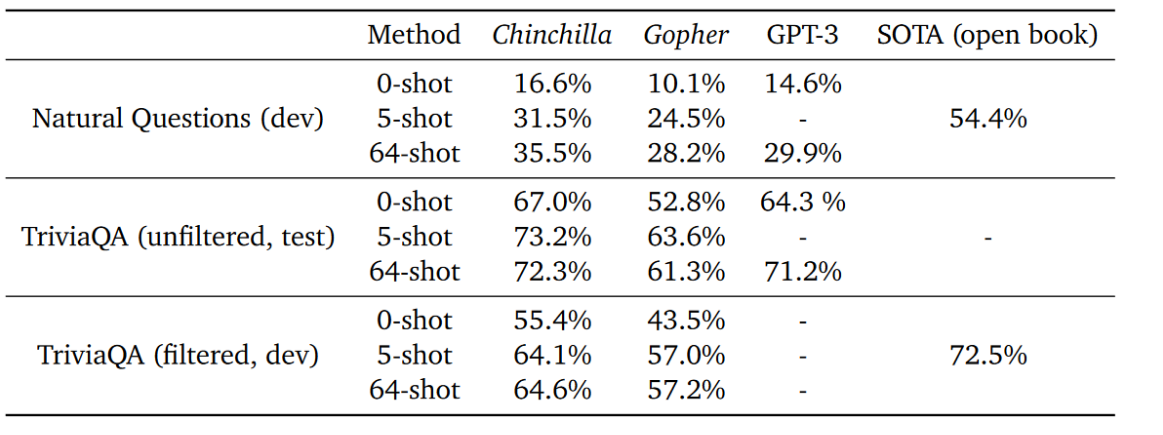
\includegraphics[width = 12cm]{./figure/chinchilla_qa.png} \\ 
	\citebutton{Source: Hoffmann et al., 2022}{https://arxiv.org/abs/2203.15556}
\end{figure}

\vfill

\end{vbframe}

% ------------------------------------------------------------------------------

\endlecture

\end{document}
